\begin{figure}[htbp]
\centering
\begin{tikzpicture}[x=1.5cm,y=1.5cm]
 \fill[black!7] (0,1)--(1,1)--
   plot[domain=1:4,samples=80] (\x,{(\x+1/\x)/2})
   --(4,2.6)--(0,2.6)--cycle;
 \draw[->] (0,0)--(4.25,0) node[right] {$r/Q$};
 \draw[->] (0,0)--(0,2.85) node[above] {$m/Q$};
 \draw[thick] (0,1)--(1,1);
 \draw[thick,domain=1:4,samples=80] plot (\x,{(\x+1/\x)/2});
 \draw[densely dotted] (1,0)--(1,2.6);
 \draw (1,.04)--(1,-.04) node[below] {$1$};
 \draw (.04,1)--(-.04,1) node[left] {$1$};
 \node at (1.95,2.15) {allowed region};
 \node[below right] at (2.4,1.18) {$m=\tfrac12(r+Q^2/r)$};
 \node[above] at (.5,1) {$m=Q$};
\end{tikzpicture}
\caption{The charged upper-area inequality for $Q>0$.
For $r\le Q$, it requires only $m\ge Q$.
For $r\ge Q$, its boundary is $m=(r+Q^2/r)/2$.
The mass-lower-bound expression must therefore be restricted to this latter branch.}
\label{fig:charged-region}
\end{figure}
